%第3章2
\section{設計}
 以下に基本設計、詳細設計を示したシステムのクラス図\cite{v_model}を図\ref{class}に載せる。
\begin{figure}[htbp]
\centering
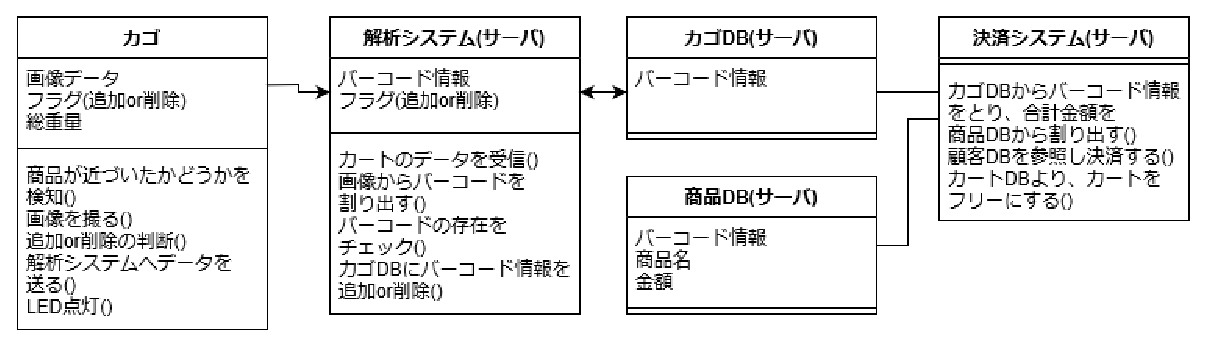
\includegraphics[width=15cm]{./pic/class_final.eps}
\caption{クラス図}
\label{class}
\end{figure}

 図\ref{class}は大きく分けてカゴ、解析システム、カゴDB、商品DB、決算システムをクラスとしたときにそれぞれが持つ属性と操作を表している。カゴはエッジ側は処理を担当し、ユーザが商品を出し入れする際にその商品の画像データを確保したりユーザに解析が成功したかの通知をするためのクラスをまとめたものである。解析システムはカゴクラスから送られてきたデータの受信、解析とカゴDBへの操作をクラスにしたものである。カゴDBは現在ユーザが購入予定の商品に何があるのかを管理する。商品DBには商品のバーコード番号と商品名、値などの商品自体の情報が管理されてある。店側が新しい商品を追加する場合はこのDBに商品情報を追加する必要がある。最後に決済システムは最終的にユーザが購入する際に必要な機能をクラスにしている。
 \ref{class}に記述されているシステムの機能について説明していく。
\begin{itemize}
\item カゴ
 カゴの属性である画像データは商品が近づいたかどうか検知する操作によって取得する。画像データ属性とフラグ(追加・削除)の2つのデータの取得が完了すると解析システムへデータを送る。ここでいうフラグの追加の役割はユーザがカゴに購入予定の商品を入れる場合にしようする。削除はすでにカゴ内にある商品の購入をやめる場合に使用する。
このフラグ(追加・削除)の判断には重量センサを用いて行う。重量センサから取得できる総重量が増えた場合は追加すると判断し、減少した場合は削除すると判断する。LED点灯は解析システム側で解析が成功した場合にユーザへの通知としての役割がある。
\item 解析システム
 カゴクラスが解析に必要な画像データとフラグ(追加・削除)を送信すると解析システムがデータを受信して解析が始まる。画像データからバーコード番号を割り出すことに成功すると一緒に受信したフラグを使用してカゴDBにバーコード番号を追加する。ただし存在しない番号を追加してしまわないようにDBに追加する前に商品DBに該当するバーコード番号があった場合のみ追加を行う。また解析に成功しても失敗してもカゴへ成否の結果を送信する。
\item カゴDB
 カゴDBはユーザの購入予定の商品のバーコード番号の管理を行う。このDBは解析システムによって操作される。また決済システムによって決済が終了した場合はデータは削除される。
\item 商品DB
 この商品DBはシステムの動作中には追加・削除などの操作は行われず、参照のみ行われる。このDBは店側が新商品の追加や値段の更新を行いたい場合に操作される。
\item 決済システム
 最後の決済システムが行うのはユーザが決済を行うときに機能する。ユーザが商品を出し入れする時点でカゴDBに購入予定の商品の情報が格納されているため決済時にカゴの中にある商品を1つずつスキャンする必要はない。つまり決済が一瞬で完了することになる。
\end{itemize}